% !TeX root = Bericht.tex
% !TeX spellcheck = de_DE
\section{Theorie}
\label{sec:theorie}
Dieses Kapitel erklärt die notwendige Theorie zum Versuch. Dabei wird am Anfang mit den wichtigen Effekten der Röntgenstrahlung begonnen, danach folgen Reflexion und Absorption an bzw. in Medien, sowie eine Erkärung der Funktionsweise eines Geiger-Müller-Zählrohrs. Kurz wird auch die Poisson-Statistik erklärt, die für die Fehleranalyse relevant ist. \cite{roentgenskript}


\subsection{Bremsstrahlung und charakteristische Röntgenstrahlung}
Bremsstrahlung nennt man den Effekt, wenn die kinetische Energie eines Elektrons in die Energie eines Photons umgewandelt wird. Dabei entsteht ein kontinuierliches Spektrum, das jedoch unterhalb einer minimalen Wellenlänge $\lambda_{\mathrm{min}}$ verschwindet, da die Maximalenergie der Elektronen durch die angelegte Anodenspannung $U_{\mathrm{A}}$ festgelegt ist. Die maximale Energie des beschleunigten Elektrons beträgt $E=e\cdot U_{\mathrm{A}}$, damit erhält man die minimale Wellenlänge 
\begin{equation}
	\lambda_{\mathrm{min}}=\frac{hc}{eU_{\mathrm{A}}}. 
\end{equation} \label{eq:Plank}
Im Gegensatz zum kontinuierlichen Spektrum der Bremsstrahlung, wird bei der charakteristischen Röntgenstrahlung ein Spektrum mit scharfen Peaks emittiert. Die Wellenlängen der Peaks hängen dabei vom Material der Anode ab. Die Energieemission ensteht dabei durch elektronische Übergänge in den Atomen der Anode. Ein hochenergetisches Elektron mit passender Wellenlänge kann dabei ein Elektron der inneren Schalen eines Anodenatoms lösen. Ein Elektron höherer Schale ersetzt das fehlende Elektron. Dabei wird, unter Vernachlässigung von Quanteneffekten wie der Feinstrukturaufspaltung, ein Photon der Energie der Differenz der beiden Schalen emittiert, also mit Energie $\Delta E=h\nu$. Die Schalen folgen der aufsteigenden Benennung K, L, M, N,…. In \autoref{roentgenspektrum_skript} ist beispielhaft ein Röntgenspektrum für Reflexionen an einem NaCl-Kristall gezeigt. In der Nomenklatur der Peaks gibt dabei der Großbuchstabe die Zielschale des Elektrons an, der griechische Buchstabe die ursprüngliche, aus welcher das Elektron war, bevor es die Lücke füllte. Ein K$_\alpha$-Übergang bedeutet also, dass ein Elektron aus der K-Schale gelöst wurde, und von einem aus der L-Schale ersetzt wird.    
\begin{figure}[H]
	\centering
	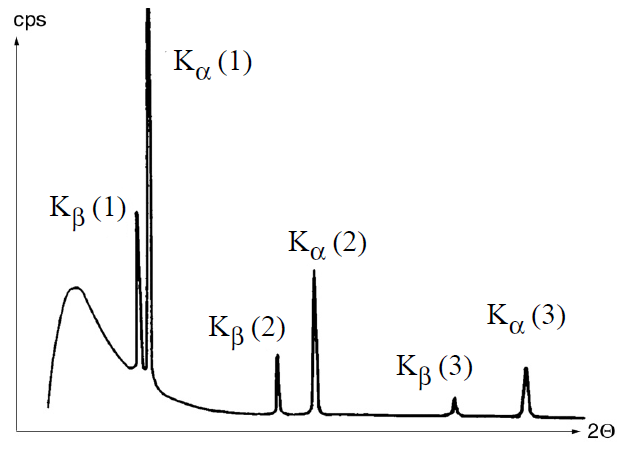
\includegraphics[width=0.6\textwidth]{roentgenspektrum_skript}
	\caption{Schematisches Röntgenspektrum für Reflexionen an einem NaCl-Kristall mit Beschriftung der Peaks der charakteristischen Röntgenstrahlung. Abbildung entnommen aus \cite{roentgenskript}. }
	\label{roentgenspektrum_skript}
\end{figure}

\subsection{Bragg-Reflexion}
Wenn Licht auf eine Kristallstruktur fällt, werden die Wellen teilweise an den verschiedenen Gitterebenen reflektiert. Um konstruktive Interferenz zu erhalten, muss der Gangunterschied zwischen den verschiedenen reflektierten Lichtwellen ein ganzzahliges Vielfaches ihrer Wellenlänge $\lambda$ sein. Dies wird auch als Bragg-Bedingung bezeichnet und ist in \autoref{bragg_schema} dargestellt.
\begin{figure}[H]
	\centering
	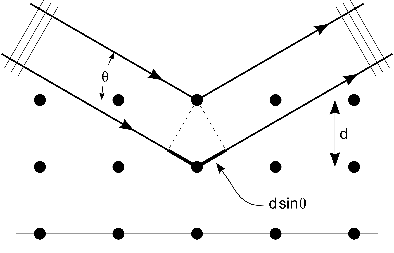
\includegraphics[width=0.6\textwidth]{bragg}
	\caption{Graphische Darstellung der Bragg-Reflexion mit eingezeichnetem Einfallswinkel $\theta$ und Reflexion an zwei Ebenen des Kristalls. Insbesondere hervorgehoben ist der Phasenunterschied zwischen den Brechungen an beiden Ebenen. Abbildung entnommen aus \cite{bragg}. }
	\label{bragg_schema}
\end{figure}


Formal besagt die Bragg-Bedingung, dass

\begin{equation}\label{eqn:bragg}
	n\lambda = 2d\sin(\theta),
\end{equation}

wobei \( d \) der Gitterebenenabstand, \( n \) eine ganze Zahl und \( \theta \) der Winkel ist, unter dem das Licht auf den Kristall fällt. 


\subsection{Absorption in Medien}
Beim Durchqueren von Materie nimmt die Intensität von Röntgenstrahlen mit der Dicke $d$ exponentiell ab, und hängt vom Absorptionskoeffizienten $\mu$ ab. Dieser Faktor ist eine Funktion der Wellenlänge der eintreffenden Welle und der Ordnungszahl der Absorberatome. Für die Intensität $I$ in Abhängigkeit der Dicke des Materials ergibt sich also
\begin{equation}\label{eqn:mu}
	I(d)=I_0\exp{(-\mu(\lambda, Z)d)},
\end{equation}
wobei $I_0$ die Intensität bevor dem Eintreten ins Material angibt. 
Gründe für diese Absorptionen sind Photoeffekt, Compton-Streuung und Paarerzeugung. Paarerzeugung benötigt höhere Energien, als in diesem Versuch verwendet werden, daher sind hier nur Photoeffekt und Compton-Streuung relevant. Der gesamte Absorptionskoeffizient wird als Summe der einzelnen Bestandteile gebildet als
\begin{equation}
	\mu=\tau_{\mathrm{Photoeffekt}}+\sigma_{\mathrm{Streuung}}.
\end{equation}
Als Nächstes wird der Massenabsorptionskoeffizient als $\mu/\rho$ definiert, wobei $\rho$ die Dichte des Absorbermaterials beschreibt. Für diesen Koeffizienten ergibt sich die Proportionalität
\begin{equation}\label{eqn:tau}
	\frac{\tau}{\rho}\sim \frac{\mu}{\rho}=k\cdot(\lambda^3Z^3)
\end{equation}
aus dem Grund, dass für die betrachteten Energien der Photoeffekt dominiert. Dabei ist zu beachten, dass der Faktor $k$ nicht für alle Wellenlängen konstant ist. Er hat für Wellenlängen $\lambda<\lambda_{\mathrm{K}}$ einen anderen Wert als für $\lambda>\lambda_{\mathrm{K}}$, wobei $\lambda_\mathrm{K}$ das Energieniveau der K-Schale ist.
\subsection{Absorptionskante}

Absorptionskanten sind sprunghafte Anstiege der Absorption beim Anstieg der Frequenz (direkt proportional zur Energie). Sie rühren aus der Tatsache her, dass Atome Röntgenphotonen erst dann absorbieren können, wenn deren Wellenlänge kleiner ist als die, welche benötigt wird, um ein Elektron in eine höhere Schale zu heben. Nach dem Passieren dieser Frequenz ändert sich auch der Absorptionskoeffizient $\mu$, da nun die Möglichkeit besteht, andere Elektronen anzuregen (vgl. \autocite{absorbtionskante}).

\subsection{Funktionsweise Geiger-Müller-Zählrohr}
Zur Messung der Anzahl an eintreffenden Röntgenquanten wird ein Geiger-Müller-Zählrohr verwendet. Dieser besteht aus einem Zähldraht, der sich in einem Zählrohrmantel befindet. Diese beiden sind mit einer Spannung verbunden, weshalb im Rohr ein elektrisches Feld erzeugt wird. Eintreffende ionisierende Strahlung erzeugt im Füllgas des Rohrs Elektron-Ion-Paare. Während die Ionen sich langsam Richtung Mantel bewegen, werden die Elektronen stark zum Draht beschleunigt. Dabei erzeugen die Elektronen auch neue Elektron-Ion-Paare, die zu einer Kaskade führen, die am Draht eintrifft. Treffen sie am Draht auf, entsteht ein Spannungspuls, der vom Zähler registriert wird. Ist die eingestellte Spannung zu gering, können viele eintreffende Elektronen nicht detektiert werden, weil sie keine Lawine auslösen können. Auf einer gewissen Spanne an Spannungen, genannt Plateau, können im Rahmen der Unsicherheit alle Elektronen registriert werden. Bei zu hohen Spannungen können Gasatome auch ohne ionisierendem Elektron ionisieren und eine Kaskade auslösen \cite{geigerzähler}. 
In \autoref{aufbau_geigerzähler} ist der schematische Aufbau eines Geiger-Müller-Zählers gezeigt. 
\begin{figure}[H]
	\centering
	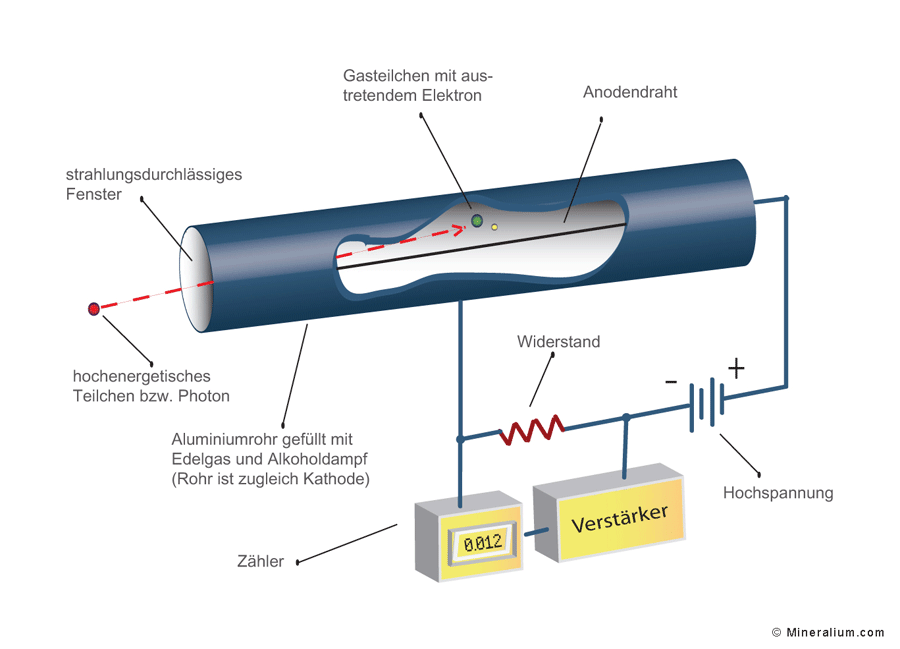
\includegraphics[width=0.9\textwidth]{geiger_mueller_zaehlrohr_abbildung}
	\caption{Schematischer Aufbau eines Geigerzählers. Dargestellt sind Anodendraht und das Kathodenrohr. Zudem sind die Anschlüsse von Spannung und Widerstand sowie der Zähler, der die Spannungspulse aufzeichnet, dargestellt. Abbildung entnommen aus \cite{geigerzähler_bildl}. }
	\label{aufbau_geigerzähler}
\end{figure}



\subsection{Poisson-Statistik}
Die Poisson-Verteilung ist eine diskrete Verteilung, die für Experimente mit abzählbarem Ergebnis verwendet wird. Dabei kann die Verteilung durch einen Erwartungswert charakterisiert werden, mit welcher Wahrscheinlichkeit gewisse Ereigniszahlen auftreten. Ein besonderes Charakteristikum der Poisson-Verteilung ist die Unsicherheit der Werte. Diese beträgt genau die Wurzel der gemessenen Anzahl, der Fehler einer Größe $N$, $\delta N$, beträgt also 
$$\delta N=\sqrt{N}. $$










%\begin{figure}[H]
%    \centering
%    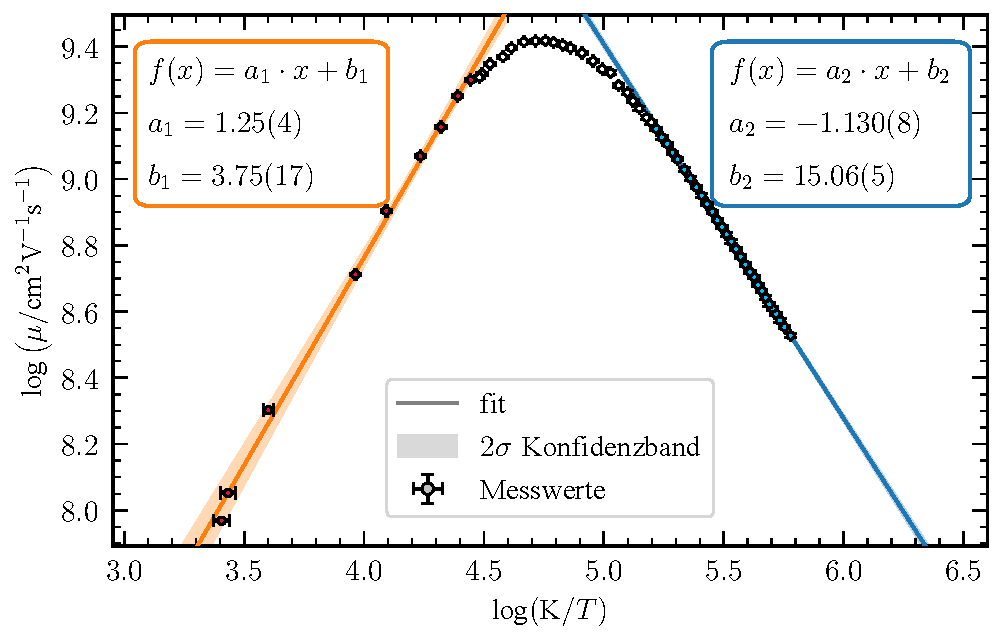
\includegraphics[width=\textwidth]{plot3.pdf}
%    \caption{}
%    \label{fig:plot3}
%\end{figure}
